\chapter{Analizadores empleados en el web scraping}
\label{cha:analizadores empleados en el web scraping}

Este apéndice tiene como objetivo introducir aquellos aspectos más relevantes relacionados con los
analizadores, también conocidos como \emph{parsers}, empleados en el web scraping. A lo largo de esta sección
se realizará una pequeña sinopsis de aquellas herramientas empleadas en los algoritmos de extracción de
los paquetes definidos en la sección \ref{sec:paquetes de python encontrados durante el proceso de 
busqueda}.

A modo de introducción cabe destacar que un analizador sintáctico, es un programa informático que analiza
una cadena de símbolos según las reglas de una gramática formal \cite{parser-wikipedia}. Generalmente, los 
analizadores se componen de dos partes, por un lado, un analizador sintáctico, y por otro un analizador 
léxico. Mientras que el analizador léxico crea tokens a partir de una secuencia de caracteres de entrada, 
el analizador sintáctico convierte los tokens en otras estructuras.

\begin{figure}[tphb]
    \centering
    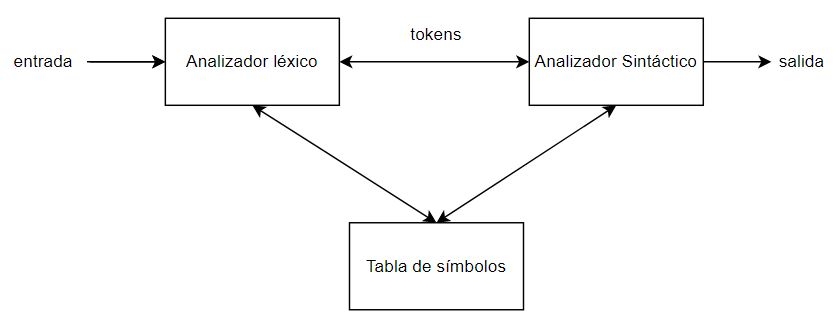
\includegraphics[width=5.5in]{parser-structure.jpg}
    \caption{Estructura basica de un analizador}
    \label{img:estructura basica de un analizador}
\end{figure}

\section{lxml}
\label{sec:lxml}

Uno de los analizadores más comunes en todos los algoritmos de minado web es \emph{lxml} \cite{lxml}. Esta
biblioteca de Python permite procesar tanto documentos XML como HTML.

Como la gran mayoría de analizadores, lxml convierte el texto de entrada en una estructura tipo árbol. Esto
permite navegar por la propia estructura en busca de la información que se desea de forma sencilla. 

En el caso del web scraping, la manera en la que lxml es capaz de encontrar información valiosa, es decir 
texto, es a través de expresiones XPath. Se muestra un pequeño ejemplo a continuación.

\begin{Schunk}
    \begin{Soutput}
        > html.xpath("string()")
        # TEXTTAIL

        > html.xpath("//text()")
        # ['TEXT', 'TAIL']
    \end{Soutput}
\end{Schunk}

Cabe destacar que el resultado dado por una expresión XPath es un objeto especial que conoce parte de su
estructura. Esto permite ejecutar operaciones sobre este elemento y saber de dónde proviene a través de
diferentes métodos.

\subsection{lxml.html}
\label{subsec:lxml.html}

¿Qué ocurre con los documentos HTML mal formados? Para este propósito, se creó lo que se conoce como
\emph{lxml.html} \cite{lxml-html}. Un paquete de Python especial para tratar con documentos HTML, el cual 
a diferencia del analizador base, proporciona una API de elementos propia de HTML, así como una serie de 
utilidades para tareas comunes de procesamiento de los mismos.

\begin{Schunk}
    \begin{Soutput}
        > broken_html = "<html><head><body><h1>page title</h3>"
        > parser = etree.HTMLParser()
        > tree   = etree.parse(StringIO(broken_html), parser)
        > result = etree.tostring(tree.getroot(), method="html")
        # <html><head></head><body><h1>page title</h1></body></html>
    \end{Soutput}
\end{Schunk}

Como se puede observar, incluso analizando documentos realmente mal formados, el analizador es capaz de
crear una estructura propia de un documento HTML. A partir de ahí, es posible aplicar expresiones XPath con
el fin de recorrer el árbol generado y recuperar información de valor.

\subsection{soupparser}
\label{subsec:soupparser}

Otro de los analizadores propios de lxml es \emph{soupparser} \cite{lxml-soup} propio del paquete
BeautifulSoup. La forma en la que lxml interactúa con BeautifulSoup, es a través del módulo 
\emph{lxml.html.soupparser} el cual proporciona una seria de funciones principales. 

Por un lado, tanto \emph{fromstring()} como \emph{parse()} se emplean para analizar ya sea una cadena o un 
archivo HTML, por otro lado \emph{convert\_tree()} se emplea para convertir un árbol BeautifulSoup existente 
en una lista de elementos de nivel superior.

\begin{Schunk}
    \begin{Soutput}
        > tag_soup = '''<meta/><head></head><body>Hi all<p>'''
        > root = fromstring(tag_soup)
        # <html><meta/><head></head><body>Hi all<p/></body></html>
    \end{Soutput}
\end{Schunk}

Imaginemos que se dispone de una cadena HTML mal formada como la mostrada en el ejemplo. Al ser una cadena,
se emplea \emph{fromstring()} para realizar un análisis de la misma. Como vemos la salida también puede
provocar algún error, puesto que no es exactamente una estructura propia de HTML.

\section{html5lib}
\label{sec:html5lib}

\emph{html5lib} \cite{html5lib} es un paquete de Python que implementa el algoritmo de análisis sintáctico 
de HTML5. Proporciona una interfaz similar a la del módulo lxml.html \ref{subsec:lxml.html} con metodos 
como \emph{fromstring()} o \emph{parse()} que operan de la misma manera que las funciones de análisis 
de HTML normales.

Al igual que lxml.html, este paquete también trabaja con árboles de objetos, pero en este caso normaliza 
algunos elementos y estructuras a un formato común. Por ejemplo, incluso si una tabla no tiene una etiqueta 
del tipo \emph{<tbody>}, se inyectará una automáticamente.

\begin{Schunk}
    \begin{Soutput}
        > tostring(html5parser.fromstring("<table><td>foo"))
        # '<table><tbody><tr><td>foo</td></tr></tbody></table>'
    \end{Soutput}
\end{Schunk}

\section{html.parser}
\label{sec:html.parser}

\emph{html.parser} \cite{html-parser} es un módulo que define una clase HTMLParse como base para analizar
archivos HTML y XHTML. Este módulo trabaja alrededor de etiquetas, pues llama a métodos de manejo cuando
se encuentran etiquetas de inicio, etiquetas finales, texto, comentarios y otros elementos de marcado.

\begin{Schunk}
    \begin{Soutput}
        > parser.feed('<p><a class=link href=#main>tag soup</p ></a>')
        # Start tag: p
        # Start tag: a
        # Data     : tag soup
        # End tag  : p
        # End tag  : a
    \end{Soutput}
\end{Schunk}

Como se puede observar, el algoritmo es capaz de detectar etiquetas tanto de apertura, como de cierre incluso
en documentos HTML mal formados como este. Esto hace que la búsqueda de información valiosa, en este caso
texto, sea sencilla.

